\documentclass[diss.tex]{subfiles}

\begin{document}
\chapter{Evaluation}
\label{chap:evaluation}
\section{Success criteria}
My original success criteria for this project were:
\begin{itemize}
	\item To have a tested library for operation-based CRDTs which represent an ordered list of characters
	\item To have 2 versions of a library which a text editor application might use to collaboratively edit a document with other similar applications over a network. One which will use a central server to pass data, and another where data is sent directly between clients.
	\item To have a library which, when used by an application, provides collaborative editing functionality with sufficiently small latency between clients to be considered `realtime'
\end{itemize}

During the course of the project, I realised that as well as providing sufficiently small latency, it was highly desirable for my library to have reasonable memory usage and reliability as well. I will now discuss to what extend these amended criteria were met.
\section{Core Library}
\subsection{Unit tests}
To have both continuous sanity-checking and more rigorous testing of how concurrency scenarios are handled, I compiled a suite of 50 unit tests as I developed the project. There were unit tests for some basic functions such as the operations for the helper structures, which checked for example that insertion and deletion worked as expected in the given scenarios. The tests focused on concurrency involved applying some events in different causal orders and checking they achieved the same result.
\subsection{CRDT Operation Latency}
To evaluate the performance of my library, I timed how long it took the \texttt{OperationQueue} to be ready to take from again after popping an operation, which corresponds to how long the operation took to perform and store. I plotted this against the length of the document at that point. For insertion, I applied 10,000 \texttt{AddRightLocal} operations sequentially to an empty list, and timed each one (figure \ref{fig:add_latencies}). For deletion, I first inserted 10,000 vertices into the list, then applied 10,000 \texttt{DeleteLocal} operations, then reversed the results, so that the first data point is deleting from a one element list (figure \ref{fig:del_latencies}).

\noindent
I broke the latency up into four parts: 
\begin{itemize}
\item \textit{Insertion} is the time it takes to apply the update to the CRDT
\item \textit{Store\_op} is the time taken to put the operations in the $opStore$
\item \textit{Network\_send} is the time taken to iterate over all connected peers and send the operation to them (for simplicity in the measurements there were no others)
\item \textit{Recovery} is the time spent checking $heldBackOps$ to see if any operations were waiting on this one to finish and if so adding them to the front of the queue (in the measurements there would be no such operations)
\end{itemize}

The time for deriving the new state after each operation has been omitted here as it is the same for all implementations, and it dominates the cost for the first two. Since we have to scan through the vertices in order to calculate the column in which the cursor should appear, this is a linear overhead in the size of the list.

% LLOrderedList
For \texttt{LLOrderedList}, we see that both times are independent of the length of the list. This is because lookup in the dictionary that maps identifiers to linked list nodes is a constant time operation, meaning so too are insertion and deletion in the linked list. The large spikes occurring for insertions are the resizing of Python's builtin dictionary. When this happens, the size is doubled, which explains why both the spacing between the spikes and their height doubles each time. This isn't seen in the deletion case, because at the point of the first measurement, 10,000 vertices have already been inserted, so the dictionary is already big enough.

% LSEQOrderedList
For \texttt{LSEQOrderedList}, the complex data structure used to house the linked list nodes offers roughly logarithmic-time lookup, so this dominates both insertion and deletion cost. As such, the graphs exhibit a roughly logarithmic shape. For insertion, there are visible \textit{chunks} of time when the cost is roughly constant, and the chunk boundaries are where some resizing is happening. The logarithmic shape is shown in more detail in figure \ref{fig:lseq_log}, where roughly a straight line emerges with a logarithmic x-axis.

% ArrOrderedList
For \texttt{ArrOrderedList}, since finding a node from its identifier involves a linear search on all the vertices, we see a linear relationship between the number of vertices and the time it takes to insert or delete.

The graphs nicely show how the asymptotic complexities of operations for different implementations - $O(1)$, $O(\log n)$ and $O(n)$ respectively - affect real-world performance. Additionally, we can see in figure \ref{fig:logs} in both implementations that the resizing operation completely dominates for larger documents, but at a length of around 45,000 characters, the resizing latency is still only around 1ms. In order to get up to a resizing latency of 0.1s (on the edge of being acceptable) requires approximately 7 more resizes ($2^7=128$). This happens every time the size doubles, so this time would be reached at $45,000 * 128 \approx 4$ million characters. As of Dec 2016, the largest wikipedia article was around 1.1MB in size, so at one byte per character this would be slightly larger than the largest Wikipedia article.


%
%
%%%%% Operation Latencies %%%%%
\begin{figure}[H]
\vspace{-3cm}
\begin{subfigure}{\linewidth}
\centering
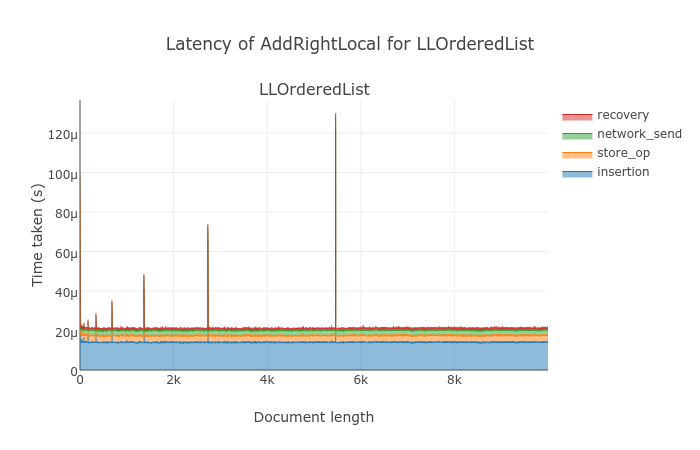
\includegraphics[height=0.25\paperheight]{add_ll}
\caption{\texttt{LLOrderedList}}
\label{fig:add_ll}
\end{subfigure}

\begin{subfigure}{\linewidth}
\centering
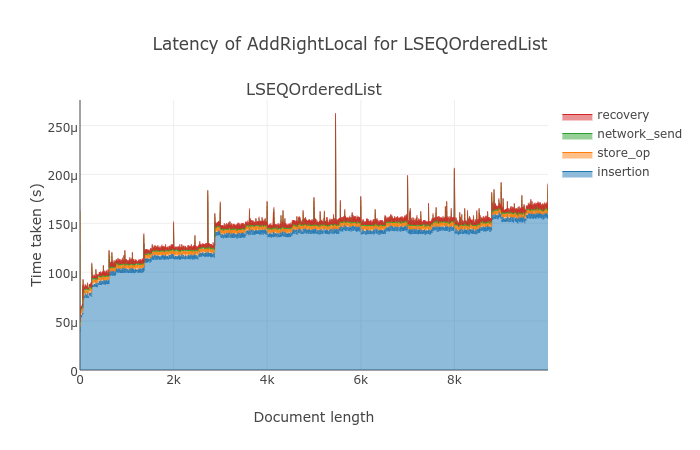
\includegraphics[height=0.25\paperheight]{add_lseq}
\caption{\texttt{LSEQOrderedList}}
\label{fig:add_lseq}
\end{subfigure}

\begin{subfigure}{\linewidth}
\centering
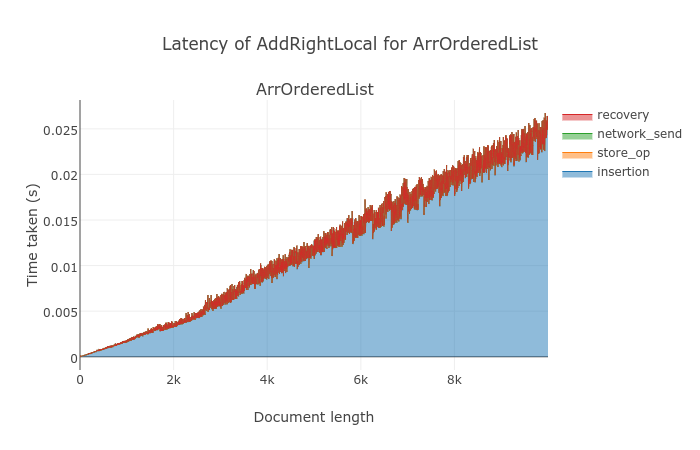
\includegraphics[height=0.25\paperheight]{add_arr}
\caption{\texttt{ArrOrderedList}}
\label{fig:add_arr}
\end{subfigure}
\caption{AddRightLocal latencies plotted against the length of the document} 
\label{fig:add_latencies}
\end{figure}
%
%
%
%
%
%
\begin{figure}
\vspace{-3cm}
\begin{subfigure}{\linewidth}
\centering
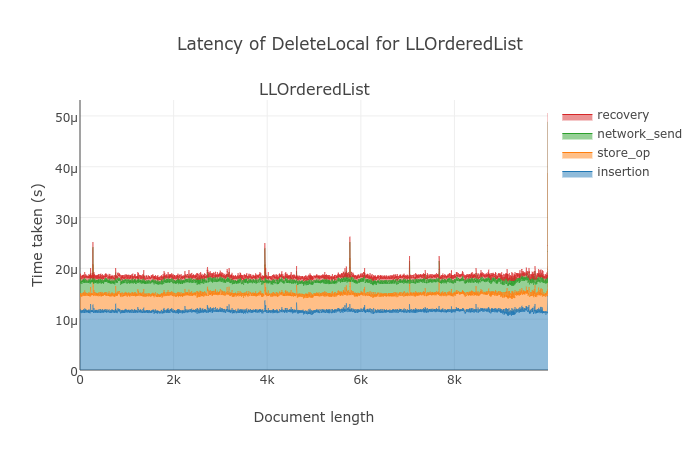
\includegraphics[height=0.25\paperheight]{del_ll}
\caption{\texttt{LLOrderedList}}
\label{fig:del_ll}
\end{subfigure}

\begin{subfigure}{\linewidth}
\centering
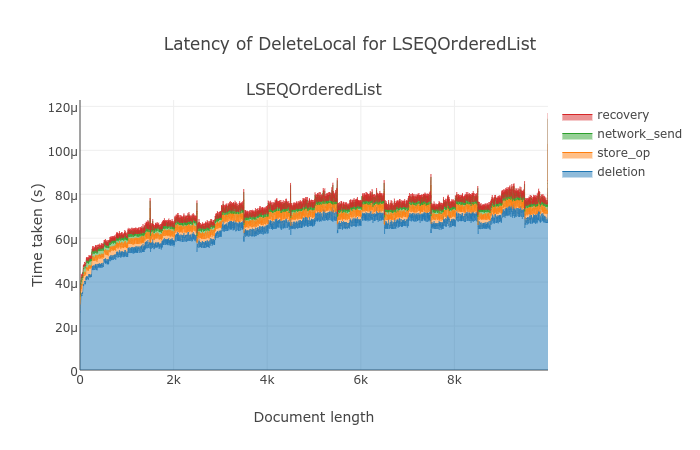
\includegraphics[height=0.25\paperheight]{del_lseq}
\caption{\texttt{LSEQOrderedList}}
\label{fig:del_lseq}
\end{subfigure}

\begin{subfigure}{\linewidth}
\centering
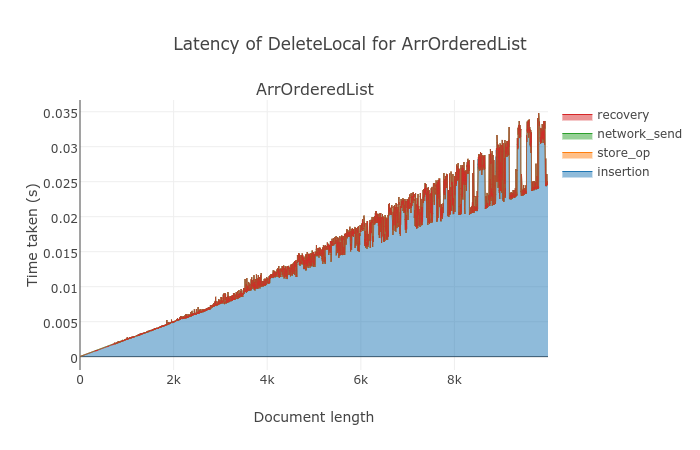
\includegraphics[height=0.25\paperheight]{del_arr}
\caption{\texttt{ArrOrderedList}}
\label{fig:del_arr}
\end{subfigure}
%
\caption{DeleteLocal latencies plotted against the length of the document} 
\label{fig:del_latencies}
\end{figure}

\begin{figure}
\begin{subfigure}{\linewidth}
\centering
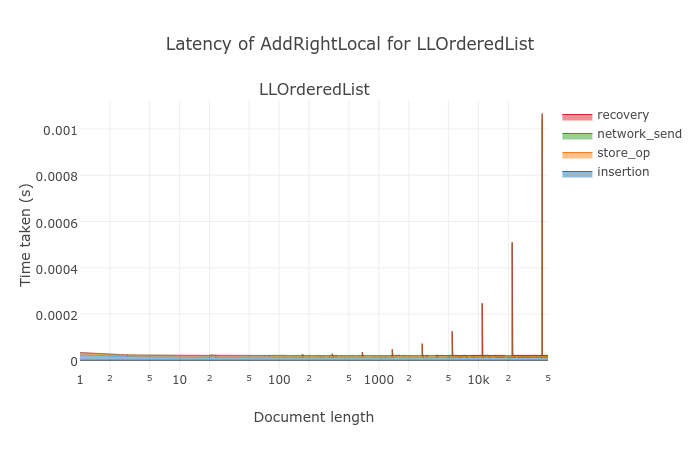
\includegraphics[height=0.25\paperheight]{add_ll_log}
\caption{A log-scale plot of insertion time for \texttt{LLOrderedList}}
\end{subfigure}

\begin{subfigure}{\linewidth}
\centering
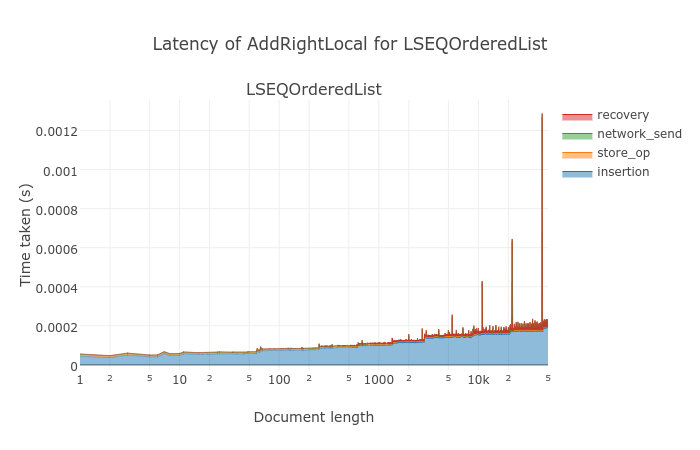
\includegraphics[height=0.25\paperheight]{add_lseq_log}
\caption{A log-scale plot of insertion time for \texttt{LSEQOrderedList}}
\end{subfigure}
%
\caption{Latency for 50,000 AddRightLocal operations on logarithmic scales}
\label{fig:logs}
\end{figure}
%
%
%
%
%
%
%
\subsection{Memory usage}
Recall that LSEQ allows vertices to be freed from memory (at the cost of more memory per vertex on average), whereas RGA allows a fixed per-vertex cost, but disallows reclaiming from memory.

To see the real-world memory usage of the different approaches, I replicated an experiment from earlier work \cite{wiki_edits} simulating editing with the revision history of different Wikipedia pages. I scraped the revisions from the pages histories, then performed a character-level \textit{diff} between consecutive versions to produce operations to transform the first version into the last that could be applied to my CRDTs.

Figure \ref{fig:wiki_edits} shows the results of this. As Figures \ref{fig:sehna} and \ref{fig:oxbridge} show, for documents with mostly insertions, the overhead of variable size identifiers outweighs not being able to delete elements. However, for documents with more deletions present, such as figure \ref{fig:wiki_admin} (a noticeboard reporting vandalous users which gets cleared when they are dealt with), we can see the non-decreasing memory usage by RGA is significantly higher. As such, choosing a scheme is a trade-off based on the expected proportion of deletions that will happen.

In the Oxbridge example, we see that for roughly 20,000 characters we are using around 200kB, which is 10 bytes per character for each identifier on average. Recalling the largest Wikipedia article to be $\sim$1.1MB in size \cite{wikilongpages} and assuming all text and 1 byte per character, my scheme would use $11 + 1.1 = 12.1$ MB to store the vertices (the largest contributor), which is a reasonable figure for an application nowadays.
%
%
%%%%% WIKI EDITS %%%%%
\begin{figure}[H]
\vspace{-3cm}

\begin{subfigure}{\linewidth}
\centering
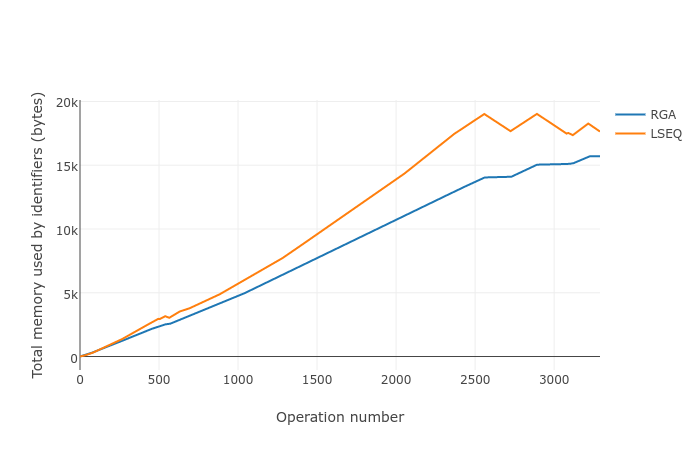
\includegraphics[height=0.25\paperheight]{Sehna}
\caption{Sehna}
\label{fig:sehna}
\end{subfigure}

\begin{subfigure}{\linewidth}
\centering
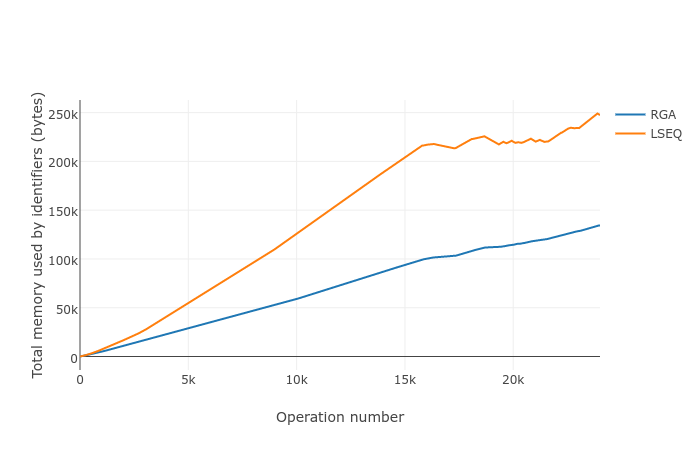
\includegraphics[height=0.25\paperheight]{Oxbridge}
\caption{Oxbridge}
\label{fig:oxbridge}
\end{subfigure}

\begin{subfigure}{\linewidth}
\centering
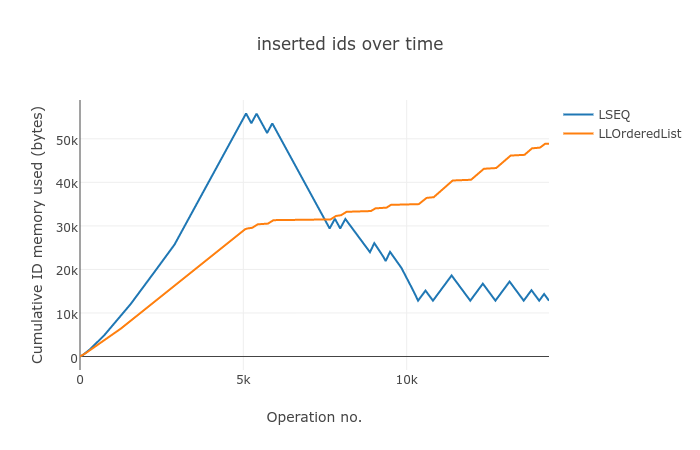
\includegraphics[height=0.25\paperheight]{Administrator_intervention_against_vandalism}
\caption{Administrator intervention against vandalism}
\label{fig:wiki_admin}
\end{subfigure}
\caption{Memory usage of my implementations of RGA (\texttt{LLOrderedList}) and LSEQ when simulating editing on Wikipedia revision history.} 
\label{fig:wiki_edits}
\end{figure}

\subsection{Undo correctness (proof)}
To show my approach to implement undo is correct, I wish to prove the following:
$$\forall l, op, n\in \mathbb{N}, others. ~length(others) = n.~ p_{undo(op)} \circ p_{others} \circ p_{op}(l)  \equiv_l p_{others}(l)$$
Where $p_x(l)$ returns the new state $l'$ obtained by performing operation $x$ on list $l$, and $others$ is a list of operations, so that $p_{others}$ is shorthand for $p_{others_0} \circ p_{others_1} \circ ... \circ p_{others_n}$. 
Let $op$ be either \texttt{Add{($v$)}} or \texttt{Delete{($v$)}} for some vertex $v$ wlog (let these be shorthand for \texttt{CRDTOpAddRightRemote}($v$) and \texttt{CRDTOpDeleteRemote}($v$) respectively).

In other words, I will show that if a replica $r$ originates an operation $op$ then performs any number of operations from other replicas, and then undoes $op$ (as the most recent operation originating from $r$ is undone), it is as if $op$ was never performed in the first place. I will prove this by induction on the length of the list $others$, $n \in \mathbb{N}$.

\noindent\underline{\textbf{Proof}}

\noindent\underline{Base case $n=0$}:\\\\
Want to show:
$$\forall l, op. ~p_{undo(op)} \circ p_{op}(l)  \equiv_l l $$

\noindent{By cases:}

\setlength{\leftskip}{1cm}

\noindent\underline{Case $op=\texttt{Add}(v)$}:\\\\
Then $undo(op) = \texttt{Delete}(v)$. Before the add, $v \notin l$ by assumption that adds are fresh. Performing the \texttt{Add} immediately followed by the \texttt{Delete} inserts then removes $v$ from the list without modifying any other vertices. Therefore, in the resulting state after both operations $l'$, $v \notin l'$ and $l \equiv_l l'$.

\noindent\underline{Case $op=\texttt{Delete}(v)$}:\\\\
Then $undo(op) = \texttt{Add}(v')$ where $v'$ differs from $v$ only in timestamp. The \texttt{Delete} followed by the \texttt{Add} removes $v$ and inserts $v'$. For $v$'s position and $rid$, there is no other vertex in $s$ already as vertices added by the same replica will be allocated different positions always (see definition of \textsc{Alloc}). So, $\nexists v''. ~ v <_v v'' <_v v'$. Thus, by the definition of $<_v$, $v'$ is inserted in the `same place' as $v$ was, and since their atoms are the same, the resulting state $l'$ is equivalent to $l$ under $\equiv_l$.

\setlength{\leftskip}{0cm}


%%%%%%%%%%%%%      IH        %%%%%%%%%%%%%%%5%%


\noindent\underline{Induction Hypothesis (IH)}:
$$\forall l, op, others. length(others) = k.~ p_{undo(op)} \circ p_{others} \circ p_{op}(l)  \equiv_l p_{others}(l) $$


%%%%%%%%%%%%%%%    Inductive step         %%%%%%%%%%%%%%%%%%%%%%%%%%%%%%%%

\noindent\underline{Inductive Step}:\\\\
Assume IH. 
Want to show $$ \forall l, op, x, others.~ length(others)=k. ~ p_{undo(op)} \circ p_x \circ p_{others} \circ p_{op}(l)  \equiv_l p_x \circ p_{others}(l) $$
%
%
\noindent or alternatively, using IH and with the same quantifications: 
$$ p_{undo(op)} \circ p_x \circ p_{others} \circ p_{op}(l)  \equiv_l  p_x \circ p_{undo(op)}\circ p_{others} \circ p_{op}(l) $$
\noindent This is shown by cases:

\setlength{\leftskip}{1cm}
\noindent Let $x$ be \texttt{Add{($v'$)}} or \texttt{Delete{($v'$)}}.

\noindent\underline{Case $v\not=v'$}:\\\\
Insertion and deletion only modify the vertex they reference in a list, so operations referencing different elements trivially commute.

\noindent\underline{Case $v=v'$}:\\\\
Then $x = \texttt{Delete}(v)$ since adds are always fresh. Now we again case split on the type of $op$:

\setlength{\leftskip}{2cm}

\noindent\underline{Case $op = \texttt{Add}(v)$}:\\\\
Then $undo(op) = \texttt{Delete}(v) = x$. Since performing a \texttt{Delete} does nothing if the vertex is already deleted, $p_{undo(op)} \circ p_x = p_x = p_x \circ p_x = p_x \circ p_{undo(op)}$ (in this context). So, $undo(op)$ and $x$ commute and we are done. 

\noindent\underline{Case $op = \texttt{Delete}(v)$}:\\\\
Then $op = x$ and since deletes are idempotent, $p_x$ is the identity function on lists, so trivially commutes with $undo(op)$ and we are done.

\setlength{\leftskip}{0cm}

\section{Networking}
\subsection{Network Latency (show latency profiles of different Tor circuit setups)}
To see how quickly operations can be delivered over the Tor network. I setup a hidden service and sent 100 operations to it from the same machine. Therefore, messages would go out to the Tor network and back in, and I would record the time of departure and arrival at my machine. Three different profiles are shown in figure \ref{fig:latency} corresponding to three different choices of circuits. The maps show the locations of the relays used in the two circuits built to the rendezvous point. As the figures show, the time spent in the network 



\subsection{Security}
A man-in-the-middle (MITM) attack describes a situation where an adversary intercepts communications along a channel and relays there own messages to each endpoint. Without the use of basic authentication for Hidden Services, my library is vulnerable to such an attack. 

% how the attack goes
To illustrate the attack, consider two peers $A$ and $B$ wanting to edit a document, and an adversary $C$ who can read and write to the channel between them. If $C$ finds out the onion address for $A$ and $B$ by some means, it can connect to $A$ and $B$. $A$ and $B$ would just assume they are connected to each other, but the key point is that the authentication is unidirectional, from $A$ to $C$ and $B$ to $C$, but not the other way round. Thus, $C$ can intercept and modify the document any way it wants. 

Basic authentication for Hidden Services, then, solves this by requiring $C$ to authenticate itself to both $A$ and $B$, by providing their specified cookies. The assumption is that these cookies are exchanged over a secure channel, such that $C$ cannot get them. However, a flaw with this system is that there is no simple revocation available. Once $C$ has a cookie, it is as authentic as any legitimate peer, and my implementation has no way to easily redistribute cookies.
\subsection{Reliability (tbd)}
\subsection{Network Architecture}
Running a P2P application instead of the client-server approach has several advantages. For example, servers are inherently bottlenecks (and single points of failure), and provide the privacy problems Google Drive poses. Decentralizing means one can potentially be completely anonymous (providing the secondary channels used to distribute onion addresses etc. preserve anonymity) as described in this project when using Tor Hidden Services, and all data completely hidden from anyone other than the specified collaborators. Moreover, the P2P mode adds no infrastructure, so its availability simply relies on the availability of the Internet and the Tor network upon which it relies.

However, the fully connected nature of the P2P approach means for $k$ connected collaborators, a new peer coming online means potentially the entire causal history of the document is sent to the new peer $k$ times (each peer may have a different set of operations so all must be queried). This is obviously wasteful as the client-server approach gives one authoritative answer.

\begin{itemize}
\item pros/cons of cl-sv vs p2p
\end{itemize}

\subsection{TODO REMOVE}



\begin{center}
!!!!!!!!!!!!!!!!!!!!!!!!!!!!!!!!!!!!!!!!!!!!!!!!!!!!!!!!!!!!!!!!!!!!!!!!!!!!!!!!!!!!!!!\\
TODO\\
!!!!!!!!!!!!!!!!!!!!!!!!!!!!!!!!!!!!!!!!!!!!!!!!!!!!!!!!!!!!!!!!!!!!!!!!!!!!!!!!!!!!!!!\\
\end{center}

\begin{itemize}
\item EXPLAIN Legend parts of timing
\item change legend for deletion not to say insertion
\item redo deletion measurements - Arr quite noisy
\item Reliability - how long
\item Tor latency
\end{itemize}



\end{document}
